\documentclass{standalone}

\newcommand{\repeatLayer}[8]{

	\foreach \i in {1,...,#7}{
		\networkLayer{#1}{#2}{#3+\i*#8+\i*#2}{#4}{#5}{};
	}

	\draw [decorate,decoration={brace,amplitude=10pt},xshift=0.4pt,yshift=-0.4pt]
	(#3+#7*#8+#7*#2+#2,#4-.2,#4+#1) -- (#3+#8+#2,#4-.2,#4+#1) node[midway,yshift=-0.6cm] {#6};
}
\usepackage{cnn, graphicx}
\usepackage{comment}

\begin{document}

\begin{tikzpicture}[scale=0.4, every node/.style={scale=1}]

	% Input
	\veclayer{
		shiftx=-2cm,
		dimy=20,%
		label/above=true,
		label/above/text=$5 \times 180$,
		label/above/y=2,
		label/below=true,
		label/below/y=2,
		label/below/text=Input,
	}

	% Tail1
	\veclayer{
		dimy=20,%
		shiftx=2cm,
		label/above=true,
		label/above/text=$5 \times 180$,
		label/above/y=2,
		label/below=true,
		label/below/y=2,
		label/below/text=Conv2D $7 \times 1 / 1$,
	}

	% Tail2
	\veclayer{
		dimy=15,%
		shiftx=4cm,
		label/above=true,
		label/above/text=$10 \times 90$,
		label/above/y=2,
		label/below=true,
		label/below/y=2,
		label/below/text=MaxPool $3 \times 1 / 2$,
	}

	% Bottleneck A
	\veclayer{
		dimy=15,%
		shiftx=7cm,
		label/above=true,
		label/above/text=$10 \times 90$,
		label/above/y=2,
		label/below=true,
		label/below/y=2,
		label/below/text=Bottleneck A,
	}

	% Downsample A
	\veclayer{
		dimy=12,%
		shiftx=9cm,
		label/above=true,
		label/above/text=$20 \times 45$,
		label/above/y=2,
		label/below=true,
		label/below/y=2,
		label/below/text=Downsample A,
	}

	% Bottleneck B
	\veclayer{
		dimy=12,%
		shiftx=13cm,
		label/above=true,
		label/above/text=$20 \times 45$,
		label/above/y=2,
		label/below=true,
		label/below/y=2,
		label/below/text=Bottleneck B,
	}

	% Downsample B
	\veclayer{
		dimy=10,%
		shiftx=15cm,
		label/above=true,
		label/above/text=$40 \times 22$,
		label/above/y=2,
		label/below=true,
		label/below/y=2,
		label/below/text=Downsample B,
	}

	% Bottleneck C
	\veclayer{
		dimy=10,%
		shiftx=19cm,
		label/above=true,
		label/above/text=$40 \times 22$,
		label/above/y=2,
		label/below=true,
		label/below/y=2,
		label/below/text=Bottleneck C,
	}

	% Downsample C
	\veclayer{
		dimy=8,%
		shiftx=21cm,
		label/above=true,
		label/above/text=$80 \times 11$,
		label/above/y=2,
		label/below=true,
		label/below/y=2,
		label/below/text=Downsample C,
	}

	% Bottleneck D
	\veclayer{
		dimy=10,%
		shiftx=25cm,
		label/above=true,
		label/above/text=$80 \times 11$,
		label/above/y=2,
		label/below=true,
		label/below/y=2,
		label/below/text=Bottleneck C,
	}

	% Downsample D
	\veclayer{
		dimy=8,%
		shiftx=27cm,
		label/above=true,
		label/above/text=$160 \times 6$,
		label/above/y=2,
		label/below=true,
		label/below/y=2,
		label/below/text=Downsample C,
	}

	% Pooling
	\veclayer{
		dimy=8,%
		shiftx=32cm,
		label/above=true,
		label/above/text=$160 \times 1$,
		label/above/y=2,
		label/below=true,
		label/below/y=2,
		label/below/text=Max/Avg Pool,
	}

	% Head
	\veclayer{
		dimy=8,%
		shiftx=34cm,
		label/above=true,
		label/above/text=$160 \times 1$,
		label/above/y=2,
		label/below=true,
		label/below/y=2,
		label/below/text=Fully Connected,
	}

	% Reg
	\veclayer{
		dimy=1,%
		densityy=1,
		densityx=1,
		densityz=1,
		shiftx=36cm,
		label/above=true,
		label/above/text=Scalar,
		label/above/y=2,
		label/below=true,
		label/below/y=2,
		label/below/text=Regression,
	}
\end{tikzpicture}

\end{document}
